\chapter{Data and Methodology}

Section about your data and the methods used.


\section{Figures}

Figures are also automatically placed and numbered. You can reference them in
the text automatically as well (see Figure~\ref{fig:example}).

\begin{figure}[h]
  \begin{center}
    % Width can be set to particular size (10cm) or relative to the page size,
    % like 0.5\textwidth (for half page) or \textwidth (for full page).
    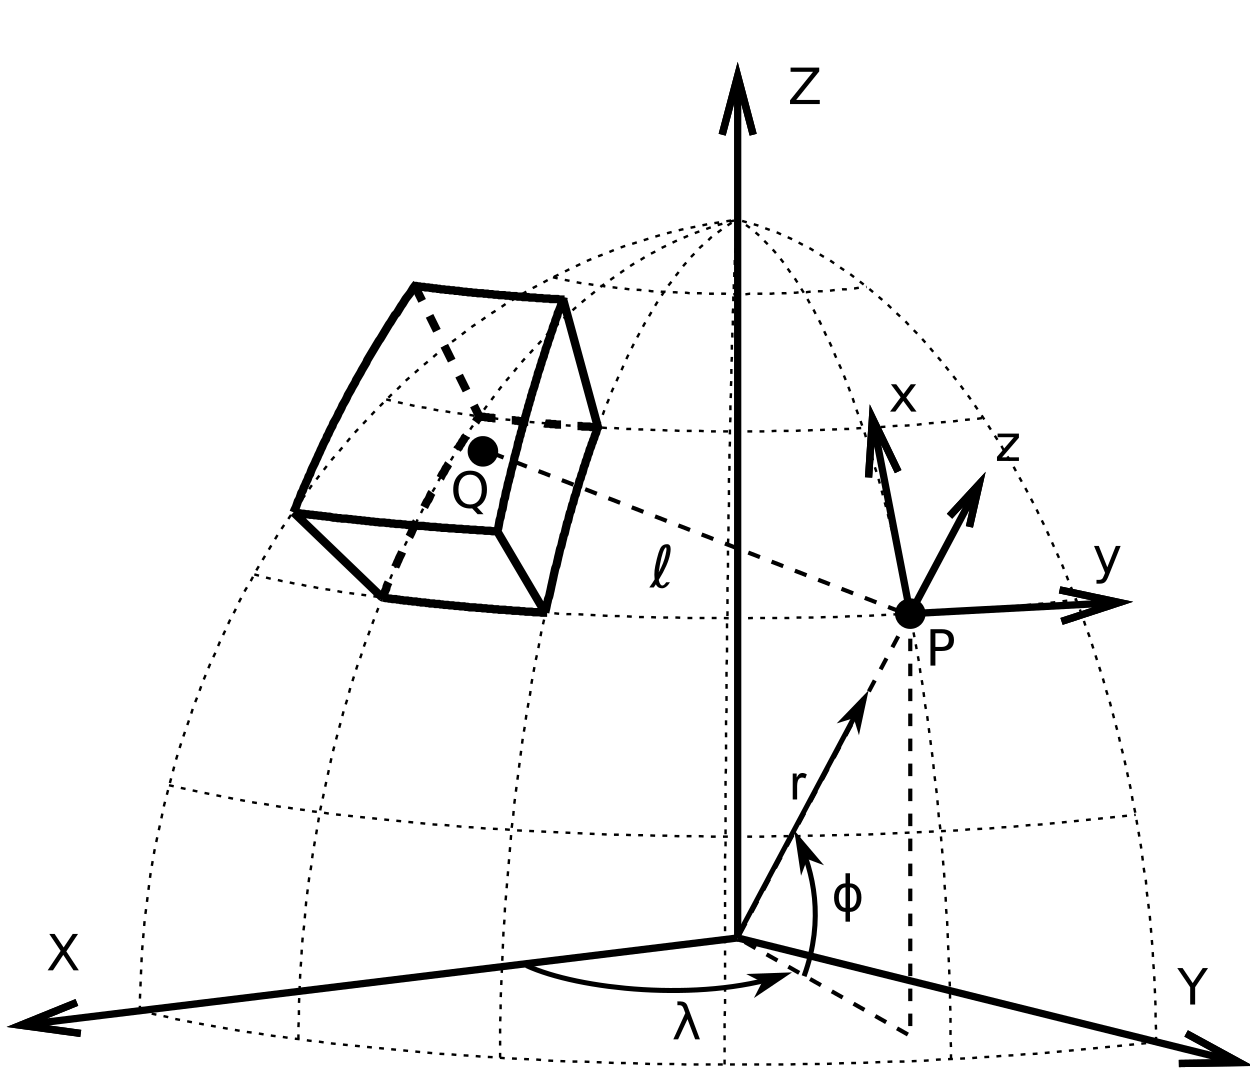
\includegraphics[width=0.5\textwidth]{figures/tesseroid-coord-sys.png}
  \end{center}
  \caption{
    This is the figure caption. Notice that the figure number is inserted into
    the text automatically. After \citet{uieda2015}.
  }
  % Label used to reference the figure in the text.
  \label{fig:example}
\end{figure}


\section{Tables}

This is an example of a table (see Table~\ref{tab:example}).

\begin{table}[h]
  \begin{center}
    % Two columns, one right aligned (r) the other centered (c)
    \begin{tabular}{rc}
      \textbf{First column}    &     \textbf{Second column}
      \\
      \hline
      Some values here  &  Others here
      \\
      Math too $\gamma = 10\ m/s^2$  &  Or not
    \end{tabular}
  \end{center}
  \caption{
    This is the table caption. Notice that the table number is inserted into
    the text automatically.
  }
  \label{tab:example}
\end{table}


\section{Equations}

This is how you can type out equations and reference them in the text. For
example, see Equation~\ref{eq:linear_least_squares} below.

\begin{equation}
  \mathbf{\hat{p}} =
    \left(\mathbf{A}^T\mathbf{A}\right)^{-1}
    \mathbf{A}^T\mathbf{d^o}
  % Label used to reference the equation in the text.
  \label{eq:linear_least_squares}
\end{equation}
